\documentclass{article}
\usepackage{qilin}
\tikzstyle{process} = [rectangle, rounded corners, minimum width=1.5cm, minimum height=0.5cm,align=center, draw=black, fill=gray!30, auto]
\title{MAT367: Differential Geometry}
\author{QiLin Xue}
\date{Fall 2021}
\usepackage{mathrsfs}
\usetikzlibrary{arrows}
\usepackage{stmaryrd}
\usepackage{accents}
\newcommand{\ubar}[1]{\underaccent{\bar}{#1}}
\usepackage{pgfplots}
\numberwithin{equation}{section}

\begin{document}

\maketitle
\tableofcontents
\newpage
\section{Manifold}
\begin{definition}
    Let $U\subset \mathbb{R}^n$, $V\subset \mathbb{R}^n$ be open. A map
    \begin{equation}
        F: U \rightarrow V
    \end{equation}
    is called \emf{smooth} if it is infinitely differentiable. The collection of all smooth maps from $U$ to $V$ is denoted as $C^\infty(U,V).$
\end{definition}
A map $F\in C^\infty(U,V)$ is a \emf{diffeomorphism} if it has a smooth inverse. For example, $e^x: \mathbb{R} \to \mathbb{R}_{>0}$ is a diffeomorphism. On the other hand, $x^3: \mathbb{R} \to \mathbb{R}$ is smooth and invertible, but its inverse is not smooth.
\begin{definition}
    Given a smooth map $F:U\to V$ and $x\in U$, its \emf{Jacobian} matrix is the $n\times m$ matrix of partial derivatives,
    \begin{equation}
        Df(x) = \left[ \frac{\partial F^i}{\partial x^j}(x)\right]_i^j.
    \end{equation} 
    If $n=m,$ the determinant of $DF(x)$ is called the \emf{Jacobian determinant.}
\end{definition}
\begin{theorem}
    \emf{Inverse Function Theorem:} A function $F:U\to V$ is a diffeomorphism if and only if,
    \begin{itemize}
        \item $F$ is invertible and smooth.
        \item $\forall x\in U$, $DF(x)$ is invertible.
    \end{itemize}
\end{theorem}
The proof is provided in MAT257.
\begin{definition}
    Let $M$ be a set.
    \begin{enumerate}[label=(\alph*)]
        \item An $m$-dimensional (coordinate) chart $(U,\varphi)$ on $M$ is a subset $U \subset M$ together with a map $\varphi: U \rightarrow \mathbb{R}^m$ such that $\varphi(U)$ is open and $\varphi$ is bijective onto its image. Here, $U$ is the \emf{chart domain} and $\varphi$ is the \emf{coordinate map.}
        \item Two charts $(U,\varphi)$ and $(V,\psi)$ are \emf{compatible} if
        \begin{enumerate}
            \item $\varphi(U \cap V)$ and $\psi(U \cap V)$ are open 
            \item $\psi \circ \varphi^{-1}: \varphi(U\cap V) \rightarrow \psi(U \cap V)$ is a diffeomorphism.
        \end{enumerate}
    \end{enumerate}
\end{definition}
Note, in MAT257, we defined coordinate charts from $\mathbb{R}^k$ to the manifold $M$. Here, it is the other way around. The definitions are equivalent since $\varphi$ is a diffeomorphism. This new perspective is interesting because we are no longer embedding $M$ into $\mathbb{R}^k$, but instead giving it a manifold structure. As a \textit{result} of this structure, we can then get a topology.
\begin{center}
    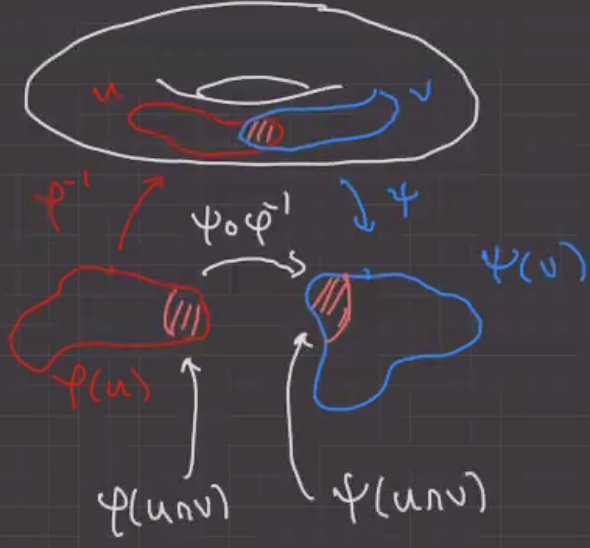
\includegraphics[width=0.4\linewidth]{L2.png}
\end{center}
Also note that if $U\cap V = \varphi$, then $(U,\varphi)$ and $(V,\psi)$ are automatically compatible.
\begin{definition}
    Given a chart $(U,\varphi)$, the composition
\begin{equation}
    U \xrightarrow[]{\varphi} \varphi(U) \subset \mathbb{R}^n \xrightarrow[]{pr^i}\mathbb{R}
\end{equation}
is equivalent to $u^i: U \rightarrow \mathbb{R}$ and are called the \emf{coordinate functions} of $\varphi$. Given $p\in U$, the $n$-tuple $(u^1(p),\dots,u^n(p))$ is called the \emf{coordinates} of $p$ in this chart. The transition maps $\psi \circ \varphi^{-1}$ are called \emf{change of coordinates.}
\end{definition}
\begin{definition}
    An $m$-dimensional \emf{atlas} on a set $M$ is a collection of coordinate charts $\mathcal{A} = \{(U_\alpha,\varphi_\alpha)\}$, such that 
    \begin{enumerate}
        \item $\bigcup_\alpha U_\alpha = M$
        \item $\forall \alpha,\beta$, $(U_\alpha,\varphi_\alpha)$ and $(U_\beta,\varphi_\beta)$ are compatible.
    \end{enumerate}
\end{definition}
Let us look at some examples.
\begin{example}
    Let $M$ be the set of \emf{affine} lines in $\mathbb{R}^n$. By affine, we mean it is just a line, and doesn't necessarily need to go through the origin. To find an atlas, define $U = \{\ell | \ell \text{ is not vertical}\}$ and $V=\{\ell | \ell \text{ is not horizontal}\}$. Any $\ell \in U$ can be written as $y=mx+b$, so the map 
    \begin{align*}
        \varphi: U &\rightarrow \mathbb{R}^2 \\ 
        y=mx+b &\mapsto (m,b)
    \end{align*}
    is a bijection. Similarly, any $\ell \in V$ can be written as $x=my+b$, so the map
    \begin{align*}
        \psi: V &\rightarrow \mathbb{R}^2 \\ 
        x=my+b &\mapsto (m,b).
    \end{align*}
    We propose that the above is an atlas. Clearly, this covers $M$ so we just need to check compatibility. Note that $U\cap V$ is the collection of lines which are not horizontal and not vertical. We have,
    \begin{align*}
        \varphi(U \cap V) &= \mathbb{R}^2 - \{\text{y-axis}\} \\ 
        &= \{(m,b): m \neq 0\},
    \end{align*}
    so it is open. Similarly, $\psi(U\cap V)$ is also open. Finally, we need to check that the transition function is a diffeomorphism, which is true since it maps
    \begin{align*}
        (m,b) &\mapsto \left(\frac{1}{m}, -\frac{b}{m}\right),
    \end{align*}
    which is smooth. Interestingly, $M$ is the \textit{infinite Mobius band.}
\end{example}
Note that we cannot simply define a manifold to be a set with an atlas. If this was true, then we could potentially have two atlases that describe a single manifold that don't necessarily agree with each other.
\begin{definition}
    Suppose that $\mathcal{A} = \{(U_\alpha, \psi_\alpha)\}$ is an $m$-dimensional atlas on $M$. Let $(U,\varphi)$ be a chart on $M$. We say that $(U,\varphi)$ is compatible with $\mathcal{A}$ if it is compatible with $(U_\alpha,\varphi_\alpha)$, for all $\alpha$.
\end{definition}
Note that $(U,\varphi)$ is compatible with $\mathcal{A}$ if and only if $\{(U,\varphi)\} \cup \mathcal{A}$ is an atlas on $M$. This implies that given any atlas, there is a \textit{maximal atlas} that contains it. We want to define $\tilde{\mathcal{A}}$ as the union of all charts which are compatible with $\mathcal{A}$. To do so, we can simply take the union of all charts that are compatible with $\mathcal{A}$. 

However, this isn't immediately obvious since the compatibility of charts is not obviously an equivalence relation. In other words, if $(U,\varphi)$ and $(V,\psi)$ are compatible with $\mathcal{A},$ are they compatible with each other? This is not true since we could get an empty triple intersection, as shown below:
\begin{center}
    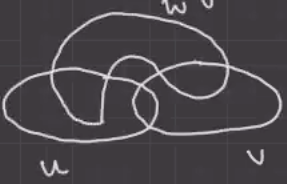
\includegraphics[width=0.4\linewidth]{L2-1.png}
\end{center}
However, since \textit{atlases} covers $M$, this is not an issue.
\begin{lemma}
    Let $\mathcal{A} = \{(U_\alpha,\varphi_\alpha)\}$ be an atlas on $M$. If $(U,\varphi)$ and $(V,\Psi)$ are compatible with $\mathcal{A}$, then they are compatible with each other.
\end{lemma}
\begin{proof}
    For every chart, the sets $\varphi_\alpha(U\cap U_\alpha)$ and $\varphi_\alpha(V \cap U_\alpha)$ are open, hence their intersection is open. This intersection is 
    \begin{align*}
        \varphi_\alpha(U\cap U_\alpha) \cap \varphi_\alpha(V \cap U_\alpha) = \varphi_\alpha(U\cap V \cap U_\alpha).
    \end{align*}
    Since $\varphi \circ \varphi_\alpha^{-1}$ is a diffeomorphism, we have that
    \begin{equation*}
        \varphi(U\cap V\cap U_\alpha) = (\varphi \circ \varphi_\alpha^{-1})(\varphi_\alpha(U\cap V \cap U_\alpha)).
    \end{equation*}
    is also open. Finally, we have that $\varphi(U\cap V) = \bigcup_\alpha \varphi(U\cap V\cap U_\alpha)$, which implies $\varphi(U\cap V)$ is open.
    
    Why is $\psi \circ \varphi^{-1}: \varphi(U\cap V) \rightarrow \psi(U\cap V)$ smooth? This is because 
    \begin{align*}
        \varphi(U\cap V\cap U_\alpha) \xrightarrow[]{\varphi_\alpha \circ \varphi^{-1}}\varphi_\alpha(U\cap V\cap U_\alpha) \xrightarrow[]{\psi \circ \varphi_\alpha^{-1}} \psi(U\cap V\cap U_\alpha).
    \end{align*}
    Therefore, $\psi\circ \varphi^{-1}\Bigg|_{U\cap V \cap U_\alpha}$ is smooth, being the composition of smooth maps. Hence, since $U_\alpha$ covers $M$, $\psi \circ \varphi^{-1}$ is smooth.
\end{proof}
\begin{theorem}
    Given an atlas $\mathcal{A}$ on $M$, let $\tilde{A}$ be the collection of all charts that are compatible with $\mathcal{A}$. Then $\mathcal{A}$ is an atlas on $M$ containing $\mathcal{A},$ and be the largest such.
\end{theorem}
\begin{definition}
    An atlas on a set $M$ is called \emf{maximal} if it is not properly contained in any larger atlas. Any atlas for $M$ determines a maximal atlas, namely $\tilde{\mathcal{A}}.$
\end{definition}
We can finally define a manifold,
\begin{definition}
    A manifold is a set $M$ together with a maximal atlas $\mathcal{A} = \{(U_\alpha, \varphi_\alpha)\}$ such that 
    \begin{enumerate}
        \item $M$ is covered by countably many charts
        \item (Hausdorff condition) For any distinct points $p,q \in M$, there are coordinate charts $(U_\alpha,\varphi_\alpha)$ and $(U_\beta,\varphi_\beta)$ such that $p \in U_\alpha$, $q\in U_\beta,$ $U_\alpha \cap U_\beta = \emptyset.$ The charts $(U_\alpha, \varphi_\alpha) \in \mathcal{A}$ are called the coordinate charts on $M$.
    \end{enumerate}
\end{definition}
Let us give some examples.
\begin{example}
    Let $M=\mathbb{R}^n$ with an atlas given by $\{(U_x,\varphi_x)\}$ where for $x\in \mathbb{R}^n$, $U_x = \{x\}$ and $\varphi_x: U_x \to \{0\} = \mathbb{R}^0$ is the unique map. This is an atlas, but fails the countability criteria.
\end{example}
\begin{example}
    Let $X= \mathbb{R} \times \{-1,1\}$ (i.e. two copies of $\mathbb{R}$). Consider the equivalence relation on $X$ generated by $(x_0,1) \sim (x_1,-1) \iff x_0 = x_1 < 0.$ This is represented by the picture below,
\begin{center}
    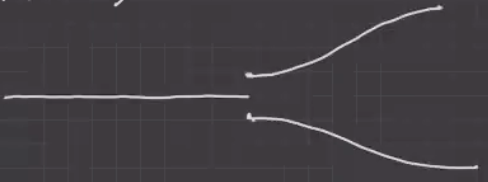
\includegraphics[width=0.4\linewidth]{L3.png}
\end{center}
    Let $M = X/\sim$. Let $\pi: X \rightarrow M$ be the quotient map, and let
    \begin{equation}
        U = \pi(\mathbb{R}\times \{1\}),\quad\quad V = \pi(\mathbb{R}\times \{-1\}).
    \end{equation}
    If $f:X\rightarrow \mathbb{R}$ defined by $(x,i) \mapsto x$, then $f$ defines a functions
    \begin{equation}
        \tilde{f}: M\rightarrow \mathbb{R}
    \end{equation}
    such that $f|_U$ and $f|_V$ are bijectors onto $\mathbb{R}$. So, $(U,f|_U)$ and $(V,f|_V)$ is an atlas on $M$ for which the Hausdoff condition fails.
\end{example}
\begin{lemma}
    Let $M$ be a set with a maximal atlas $\mathcal{A} = \{(U_\alpha, \varphi_\alpha)\}$ and suppose that $p,q \in M$ are distinct points contained in a single chart $(U,\varphi).$ Then there exists $\alpha,\beta$ such that 
    \begin{enumerate}
        \item $p\in U_\alpha$, $q\in U_\beta$
        \item $U_\alpha \cap U_\beta = \emptyset$
    \end{enumerate}
\end{lemma}
\end{document}